\documentclass[twoside]{book}

% Packages required by doxygen
\usepackage{fixltx2e}
\usepackage{calc}
\usepackage{doxygen}
\usepackage[export]{adjustbox} % also loads graphicx
\usepackage{graphicx}
\usepackage[utf8]{inputenc}
\usepackage{makeidx}
\usepackage{multicol}
\usepackage{multirow}
\PassOptionsToPackage{warn}{textcomp}
\usepackage{textcomp}
\usepackage[nointegrals]{wasysym}
\usepackage[table]{xcolor}

% Font selection
\usepackage[T1]{fontenc}
\usepackage[scaled=.90]{helvet}
\usepackage{courier}
\usepackage{amssymb}
\usepackage{sectsty}
\renewcommand{\familydefault}{\sfdefault}
\allsectionsfont{%
  \fontseries{bc}\selectfont%
  \color{darkgray}%
}
\renewcommand{\DoxyLabelFont}{%
  \fontseries{bc}\selectfont%
  \color{darkgray}%
}
\newcommand{\+}{\discretionary{\mbox{\scriptsize$\hookleftarrow$}}{}{}}

% Page & text layout
\usepackage{geometry}
\geometry{%
  a4paper,%
  top=2.5cm,%
  bottom=2.5cm,%
  left=2.5cm,%
  right=2.5cm%
}
\tolerance=750
\hfuzz=15pt
\hbadness=750
\setlength{\emergencystretch}{15pt}
\setlength{\parindent}{0cm}
\setlength{\parskip}{3ex plus 2ex minus 2ex}
\makeatletter
\renewcommand{\paragraph}{%
  \@startsection{paragraph}{4}{0ex}{-1.0ex}{1.0ex}{%
    \normalfont\normalsize\bfseries\SS@parafont%
  }%
}
\renewcommand{\subparagraph}{%
  \@startsection{subparagraph}{5}{0ex}{-1.0ex}{1.0ex}{%
    \normalfont\normalsize\bfseries\SS@subparafont%
  }%
}
\makeatother

% Headers & footers
\usepackage{fancyhdr}
\pagestyle{fancyplain}
\fancyhead[LE]{\fancyplain{}{\bfseries\thepage}}
\fancyhead[CE]{\fancyplain{}{}}
\fancyhead[RE]{\fancyplain{}{\bfseries\leftmark}}
\fancyhead[LO]{\fancyplain{}{\bfseries\rightmark}}
\fancyhead[CO]{\fancyplain{}{}}
\fancyhead[RO]{\fancyplain{}{\bfseries\thepage}}
\fancyfoot[LE]{\fancyplain{}{}}
\fancyfoot[CE]{\fancyplain{}{}}
\fancyfoot[RE]{\fancyplain{}{\bfseries\scriptsize Generated by Doxygen }}
\fancyfoot[LO]{\fancyplain{}{\bfseries\scriptsize Generated by Doxygen }}
\fancyfoot[CO]{\fancyplain{}{}}
\fancyfoot[RO]{\fancyplain{}{}}
\renewcommand{\footrulewidth}{0.4pt}
\renewcommand{\chaptermark}[1]{%
  \markboth{#1}{}%
}
\renewcommand{\sectionmark}[1]{%
  \markright{\thesection\ #1}%
}

% Indices & bibliography
\usepackage{natbib}
\usepackage[titles]{tocloft}
\setcounter{tocdepth}{3}
\setcounter{secnumdepth}{5}
\makeindex

% Hyperlinks (required, but should be loaded last)
\usepackage{ifpdf}
\ifpdf
  \usepackage[pdftex,pagebackref=true]{hyperref}
\else
  \usepackage[ps2pdf,pagebackref=true]{hyperref}
\fi
\hypersetup{%
  colorlinks=true,%
  linkcolor=blue,%
  citecolor=blue,%
  unicode%
}

% Custom commands
\newcommand{\clearemptydoublepage}{%
  \newpage{\pagestyle{empty}\cleardoublepage}%
}

\usepackage{caption}
\captionsetup{labelsep=space,justification=centering,font={bf},singlelinecheck=off,skip=4pt,position=top}

%===== C O N T E N T S =====

\begin{document}

% Titlepage & ToC
\hypersetup{pageanchor=false,
             bookmarksnumbered=true,
             pdfencoding=unicode
            }
\pagenumbering{alph}
\begin{titlepage}
\vspace*{7cm}
\begin{center}%
{\Large Sogyrolib }\\
\vspace*{1cm}
{\large Generated by Doxygen 1.8.13}\\
\end{center}
\end{titlepage}
\clearemptydoublepage
\pagenumbering{roman}
\tableofcontents
\clearemptydoublepage
\pagenumbering{arabic}
\hypersetup{pageanchor=true}

%--- Begin generated contents ---
\chapter{I\+P\+A\+SS Sogyrolib \& Matrix\+Engine}
\label{index}\hypertarget{index}{}I\+P\+A\+SS Project Hoge School Utrecht H\+BO I\+C\+T-\/\+TI

Library for the {\bfseries L3\+G4200D} gryoscope and the {\bfseries M\+H7219 Led Matrix} including a Game making toolset.

By Peter Schenkels 2019





\subsection*{Description Matrix\+Engine\+:}

Interface and {\bfseries game making toolset} for the {\bfseries M\+H7219 Led Matrix chip} and other {\bfseries Hwlib Window peripherals}. This toolset includes a {\bfseries physics engine}, {\bfseries render engine}, {\bfseries collision detection}, {\bfseries camera movement} and more. Connect {\bfseries multiple M\+H7219 chips} via {\bfseries S\+PI} on the {\bfseries Arduino}. The toolset can also be used to run games inside the {\bfseries terminal}. (linux only)

\subsubsection*{How to use it\+:}

{\bfseries Hwlib} is needed for this project, consult this page for more {\bfseries information}\+: \href{https://github.com/wovo/installers}{\tt https\+://github.\+com/wovo/installers}

This library comes with a {\bfseries demo} file that is also connected to {\bfseries Sogyro lib}. But it can also be run without gyroscope (if you remove the gyroscope you wont be able to move the character).

See the Doxygen documentation for more information on how to use this library.

\subsubsection*{What you need\+:}


\begin{DoxyItemize}
\item Arduino Due (Master)
\item M\+H7219 Led Matrix Chip(s)
\end{DoxyItemize}

optional\+: Hwlib Window Peripherals such as an oled. 
\chapter{Hierarchical Index}
\section{Class Hierarchy}
This inheritance list is sorted roughly, but not completely, alphabetically\+:\begin{DoxyCompactList}
\item \contentsline{section}{field}{\pageref{classfield}}{}
\item \contentsline{section}{object}{\pageref{classobject}}{}
\begin{DoxyCompactList}
\item \contentsline{section}{entity}{\pageref{classentity}}{}
\begin{DoxyCompactList}
\item \contentsline{section}{player}{\pageref{classplayer}}{}
\end{DoxyCompactList}
\item \contentsline{section}{obstacle}{\pageref{classobstacle}}{}
\item \contentsline{section}{window}{\pageref{classwindow}}{}
\end{DoxyCompactList}
\item \contentsline{section}{physbox}{\pageref{classphysbox}}{}
\item \contentsline{section}{pos\+Touch}{\pageref{classposTouch}}{}
\item window\begin{DoxyCompactList}
\item \contentsline{section}{led\+\_\+matrix}{\pageref{classled__matrix}}{}
\end{DoxyCompactList}
\item \contentsline{section}{xy}{\pageref{classxy}}{}
\item \contentsline{section}{xyz}{\pageref{classxyz}}{}
\end{DoxyCompactList}

\chapter{Class Index}
\section{Class List}
Here are the classes, structs, unions and interfaces with brief descriptions\+:\begin{DoxyCompactList}
\item\contentsline{section}{\hyperlink{classentity}{entity} \\*A visable entity }{\pageref{classentity}}{}
\item\contentsline{section}{\hyperlink{classfield}{field} \\*Entire playground of the scene }{\pageref{classfield}}{}
\item\contentsline{section}{\hyperlink{classled__matrix}{led\+\_\+matrix} \\*Interface for the M\+H7219 led matrix chip }{\pageref{classled__matrix}}{}
\item\contentsline{section}{\hyperlink{classobject}{object} \\*A void object with a position }{\pageref{classobject}}{}
\item\contentsline{section}{\hyperlink{classobstacle}{obstacle} \\*Solid Object with a start end point }{\pageref{classobstacle}}{}
\item\contentsline{section}{\hyperlink{classphysbox}{physbox} \\*Physics engine }{\pageref{classphysbox}}{}
\item\contentsline{section}{\hyperlink{classplayer}{player} \\*Inherited class solely made for the frog jump demo }{\pageref{classplayer}}{}
\item\contentsline{section}{\hyperlink{classposTouch}{pos\+Touch} \\*Collision A\+DT }{\pageref{classposTouch}}{}
\item\contentsline{section}{\hyperlink{classwindow}{window} \\*Renders all data within the sizes and positions }{\pageref{classwindow}}{}
\item\contentsline{section}{\hyperlink{classxy}{xy} \\*2D postion A\+DT }{\pageref{classxy}}{}
\item\contentsline{section}{\hyperlink{classxyz}{xyz} \\*3D postion A\+DT }{\pageref{classxyz}}{}
\end{DoxyCompactList}

\chapter{File Index}
\section{File List}
Here is a list of all documented files with brief descriptions\+:\begin{DoxyCompactList}
\item\contentsline{section}{src/\+Sogyrolib/\+Master/\hyperlink{controller_8hpp}{controller.\+hpp} }{\pageref{controller_8hpp}}{}
\item\contentsline{section}{src/\+Sogyrolib/\+Master/\hyperlink{l3g4__master_8hpp}{l3g4\+\_\+master.\+hpp} }{\pageref{l3g4__master_8hpp}}{}
\item\contentsline{section}{src/\+Sogyrolib/\+Slave/\hyperlink{i2c__fast_8hpp}{i2c\+\_\+fast.\+hpp} }{\pageref{i2c__fast_8hpp}}{}
\item\contentsline{section}{src/\+Sogyrolib/\+Slave/\hyperlink{l3g4200_8hpp}{l3g4200.\+hpp} }{\pageref{l3g4200_8hpp}}{}
\item\contentsline{section}{src/\+Sogyrolib/\+Slave/\hyperlink{slave_8hpp}{slave.\+hpp} }{\pageref{slave_8hpp}}{}
\end{DoxyCompactList}

\chapter{Class Documentation}
\hypertarget{classcontroller}{}\section{controller Class Reference}
\label{classcontroller}\index{controller@{controller}}


Gyroscope decorator.  




{\ttfamily \#include $<$controller.\+hpp$>$}



Inheritance diagram for controller\+:
\nopagebreak
\begin{figure}[H]
\begin{center}
\leavevmode
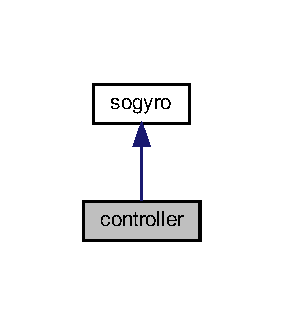
\includegraphics[width=136pt]{classcontroller__inherit__graph}
\end{center}
\end{figure}


Collaboration diagram for controller\+:
\nopagebreak
\begin{figure}[H]
\begin{center}
\leavevmode
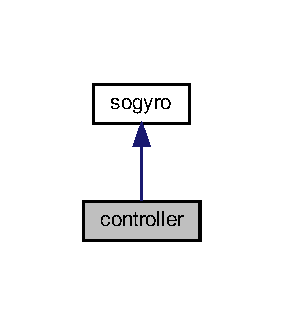
\includegraphics[width=136pt]{classcontroller__coll__graph}
\end{center}
\end{figure}
\subsection*{Public Member Functions}
\begin{DoxyCompactItemize}
\item 
\hyperlink{classcontroller_afdfd96f893a363a81df69f9011772948}{controller} (\hyperlink{classsogyro}{sogyro} \&gyro)
\begin{DoxyCompactList}\small\item\em Constructor for gyroscope decorator. \end{DoxyCompactList}\item 
int \hyperlink{classcontroller_a08706a1d0b65e1e75cd136205861c3bb}{dir} (int gyro, int scale)
\begin{DoxyCompactList}\small\item\em Returns direction as an int. \end{DoxyCompactList}\item 
int \hyperlink{classcontroller_a0f32b7bba7ac0026bbdcde8de15eeb73}{get\+\_\+dir\+\_\+x} (int scale)
\begin{DoxyCompactList}\small\item\em Returns direction x as an int. \end{DoxyCompactList}\item 
int \hyperlink{classcontroller_a6947eb778084e6c5b74b993f0fda3eaf}{get\+\_\+dir\+\_\+y} (int scale)
\begin{DoxyCompactList}\small\item\em Returns direction y as an int. \end{DoxyCompactList}\item 
int \hyperlink{classcontroller_a26c377443455cda82579776db7e2b404}{get\+\_\+dir\+\_\+z} (int scale)
\begin{DoxyCompactList}\small\item\em Returns direction z as an int. \end{DoxyCompactList}\end{DoxyCompactItemize}


\subsection{Detailed Description}
Gyroscope decorator. 

This class a decorator for the gryoscope and can be used in games. It can return values based on the tilt of the gyroscope. 

\subsection{Constructor \& Destructor Documentation}
\mbox{\Hypertarget{classcontroller_afdfd96f893a363a81df69f9011772948}\label{classcontroller_afdfd96f893a363a81df69f9011772948}} 
\index{controller@{controller}!controller@{controller}}
\index{controller@{controller}!controller@{controller}}
\subsubsection{\texorpdfstring{controller()}{controller()}}
{\footnotesize\ttfamily controller\+::controller (\begin{DoxyParamCaption}\item[{\hyperlink{classsogyro}{sogyro} \&}]{gyro }\end{DoxyParamCaption})\hspace{0.3cm}{\ttfamily [inline]}}



Constructor for gyroscope decorator. 

thsi contructor interfaces the controller decorator for the gyroscope. 

\subsection{Member Function Documentation}
\mbox{\Hypertarget{classcontroller_a08706a1d0b65e1e75cd136205861c3bb}\label{classcontroller_a08706a1d0b65e1e75cd136205861c3bb}} 
\index{controller@{controller}!dir@{dir}}
\index{dir@{dir}!controller@{controller}}
\subsubsection{\texorpdfstring{dir()}{dir()}}
{\footnotesize\ttfamily int controller\+::dir (\begin{DoxyParamCaption}\item[{int}]{gyro,  }\item[{int}]{scale }\end{DoxyParamCaption})\hspace{0.3cm}{\ttfamily [inline]}}



Returns direction as an int. 

Returns direction as an int 0 is middle 1 is right -\/1 left \mbox{\Hypertarget{classcontroller_a0f32b7bba7ac0026bbdcde8de15eeb73}\label{classcontroller_a0f32b7bba7ac0026bbdcde8de15eeb73}} 
\index{controller@{controller}!get\+\_\+dir\+\_\+x@{get\+\_\+dir\+\_\+x}}
\index{get\+\_\+dir\+\_\+x@{get\+\_\+dir\+\_\+x}!controller@{controller}}
\subsubsection{\texorpdfstring{get\+\_\+dir\+\_\+x()}{get\_dir\_x()}}
{\footnotesize\ttfamily int controller\+::get\+\_\+dir\+\_\+x (\begin{DoxyParamCaption}\item[{int}]{scale }\end{DoxyParamCaption})\hspace{0.3cm}{\ttfamily [inline]}}



Returns direction x as an int. 

Returns direction x as an int 0 is middle 1 is right -\/1 left \mbox{\Hypertarget{classcontroller_a6947eb778084e6c5b74b993f0fda3eaf}\label{classcontroller_a6947eb778084e6c5b74b993f0fda3eaf}} 
\index{controller@{controller}!get\+\_\+dir\+\_\+y@{get\+\_\+dir\+\_\+y}}
\index{get\+\_\+dir\+\_\+y@{get\+\_\+dir\+\_\+y}!controller@{controller}}
\subsubsection{\texorpdfstring{get\+\_\+dir\+\_\+y()}{get\_dir\_y()}}
{\footnotesize\ttfamily int controller\+::get\+\_\+dir\+\_\+y (\begin{DoxyParamCaption}\item[{int}]{scale }\end{DoxyParamCaption})\hspace{0.3cm}{\ttfamily [inline]}}



Returns direction y as an int. 

Returns direction y as an int 0 is middle 1 is right -\/1 left \mbox{\Hypertarget{classcontroller_a26c377443455cda82579776db7e2b404}\label{classcontroller_a26c377443455cda82579776db7e2b404}} 
\index{controller@{controller}!get\+\_\+dir\+\_\+z@{get\+\_\+dir\+\_\+z}}
\index{get\+\_\+dir\+\_\+z@{get\+\_\+dir\+\_\+z}!controller@{controller}}
\subsubsection{\texorpdfstring{get\+\_\+dir\+\_\+z()}{get\_dir\_z()}}
{\footnotesize\ttfamily int controller\+::get\+\_\+dir\+\_\+z (\begin{DoxyParamCaption}\item[{int}]{scale }\end{DoxyParamCaption})\hspace{0.3cm}{\ttfamily [inline]}}



Returns direction z as an int. 

Returns direction z as an int 0 is middle 1 is right -\/1 left 

The documentation for this class was generated from the following file\+:\begin{DoxyCompactItemize}
\item 
src/\+Sogyrolib/\+Master/\hyperlink{controller_8hpp}{controller.\+hpp}\end{DoxyCompactItemize}

\hypertarget{classi2c__fast}{}\section{i2c\+\_\+fast Class Reference}
\label{classi2c__fast}\index{i2c\+\_\+fast@{i2c\+\_\+fast}}


hwlib\+::i2c\+\_\+bus\+\_\+bit\+\_\+banged\+\_\+scl\+\_\+sda Decorator  




{\ttfamily \#include $<$i2c\+\_\+fast.\+hpp$>$}



Inheritance diagram for i2c\+\_\+fast\+:
\nopagebreak
\begin{figure}[H]
\begin{center}
\leavevmode
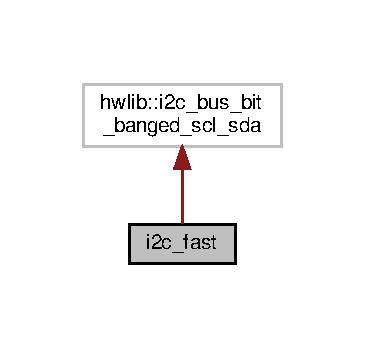
\includegraphics[width=175pt]{classi2c__fast__inherit__graph}
\end{center}
\end{figure}


Collaboration diagram for i2c\+\_\+fast\+:
\nopagebreak
\begin{figure}[H]
\begin{center}
\leavevmode
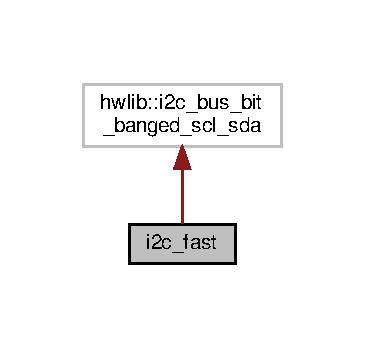
\includegraphics[width=175pt]{classi2c__fast__coll__graph}
\end{center}
\end{figure}
\subsection*{Public Member Functions}
\begin{DoxyCompactItemize}
\item 
\hyperlink{classi2c__fast_a2409918a4b030ad310e9b145e1056eb2}{i2c\+\_\+fast} (hwlib\+::i2c\+\_\+bus\+\_\+bit\+\_\+banged\+\_\+scl\+\_\+sda \&bus, uint8\+\_\+t \&address)
\begin{DoxyCompactList}\small\item\em Constructor of hwlib\+::i2c\+\_\+bus\+\_\+bit\+\_\+banged\+\_\+scl\+\_\+sda Decorator. \end{DoxyCompactList}\item 
uint8\+\_\+t \hyperlink{classi2c__fast_a90f3dca1f0688fc2ae567c6ee8b6c42e}{read} (uint8\+\_\+t \&data)
\begin{DoxyCompactList}\small\item\em Writes data from givin byte to read data into givin byte. \end{DoxyCompactList}\item 
uint8\+\_\+t \hyperlink{classi2c__fast_a51ad18b2edee256e274ee8f014369b73}{read} (uint8\+\_\+t \&register\+\_\+address, uint8\+\_\+t \&storage)
\begin{DoxyCompactList}\small\item\em Writes data from register byte byte to read data into givin storage byte. \end{DoxyCompactList}\end{DoxyCompactItemize}


\subsection{Detailed Description}
hwlib\+::i2c\+\_\+bus\+\_\+bit\+\_\+banged\+\_\+scl\+\_\+sda Decorator 

This class is hwlib\+::i2c\+\_\+bus\+\_\+bit\+\_\+banged\+\_\+scl\+\_\+sda Decorator used to write shorter lines of codes to write and read bytes with a givin address. 

\subsection{Constructor \& Destructor Documentation}
\mbox{\Hypertarget{classi2c__fast_a2409918a4b030ad310e9b145e1056eb2}\label{classi2c__fast_a2409918a4b030ad310e9b145e1056eb2}} 
\index{i2c\+\_\+fast@{i2c\+\_\+fast}!i2c\+\_\+fast@{i2c\+\_\+fast}}
\index{i2c\+\_\+fast@{i2c\+\_\+fast}!i2c\+\_\+fast@{i2c\+\_\+fast}}
\subsubsection{\texorpdfstring{i2c\+\_\+fast()}{i2c\_fast()}}
{\footnotesize\ttfamily i2c\+\_\+fast\+::i2c\+\_\+fast (\begin{DoxyParamCaption}\item[{hwlib\+::i2c\+\_\+bus\+\_\+bit\+\_\+banged\+\_\+scl\+\_\+sda \&}]{bus,  }\item[{uint8\+\_\+t \&}]{address }\end{DoxyParamCaption})\hspace{0.3cm}{\ttfamily [inline]}}



Constructor of hwlib\+::i2c\+\_\+bus\+\_\+bit\+\_\+banged\+\_\+scl\+\_\+sda Decorator. 

This is the constructor of the hwlib\+::i2c\+\_\+bus\+\_\+bit\+\_\+banged\+\_\+scl\+\_\+sda Decorator, this constructor initialises the i2c\+\_\+bus and givin address. 

\subsection{Member Function Documentation}
\mbox{\Hypertarget{classi2c__fast_a90f3dca1f0688fc2ae567c6ee8b6c42e}\label{classi2c__fast_a90f3dca1f0688fc2ae567c6ee8b6c42e}} 
\index{i2c\+\_\+fast@{i2c\+\_\+fast}!read@{read}}
\index{read@{read}!i2c\+\_\+fast@{i2c\+\_\+fast}}
\subsubsection{\texorpdfstring{read()}{read()}\hspace{0.1cm}{\footnotesize\ttfamily [1/2]}}
{\footnotesize\ttfamily uint8\+\_\+t i2c\+\_\+fast\+::read (\begin{DoxyParamCaption}\item[{uint8\+\_\+t \&}]{data }\end{DoxyParamCaption})\hspace{0.3cm}{\ttfamily [inline]}}



Writes data from givin byte to read data into givin byte. 

This function writes data from givin byte to read data into givin byte \mbox{\Hypertarget{classi2c__fast_a51ad18b2edee256e274ee8f014369b73}\label{classi2c__fast_a51ad18b2edee256e274ee8f014369b73}} 
\index{i2c\+\_\+fast@{i2c\+\_\+fast}!read@{read}}
\index{read@{read}!i2c\+\_\+fast@{i2c\+\_\+fast}}
\subsubsection{\texorpdfstring{read()}{read()}\hspace{0.1cm}{\footnotesize\ttfamily [2/2]}}
{\footnotesize\ttfamily uint8\+\_\+t i2c\+\_\+fast\+::read (\begin{DoxyParamCaption}\item[{uint8\+\_\+t \&}]{register\+\_\+address,  }\item[{uint8\+\_\+t \&}]{storage }\end{DoxyParamCaption})\hspace{0.3cm}{\ttfamily [inline]}}



Writes data from register byte byte to read data into givin storage byte. 

This function writes data from register address byte to read data into givin storage byte. 

The documentation for this class was generated from the following file\+:\begin{DoxyCompactItemize}
\item 
src/\+Sogyrolib/\+Slave/\hyperlink{i2c__fast_8hpp}{i2c\+\_\+fast.\+hpp}\end{DoxyCompactItemize}

\hypertarget{classl3g4200}{}\section{l3g4200 Class Reference}
\label{classl3g4200}\index{l3g4200@{l3g4200}}


interface for \hyperlink{classl3g4200}{l3g4200}  




{\ttfamily \#include $<$l3g4200.\+hpp$>$}



Collaboration diagram for l3g4200\+:
\nopagebreak
\begin{figure}[H]
\begin{center}
\leavevmode
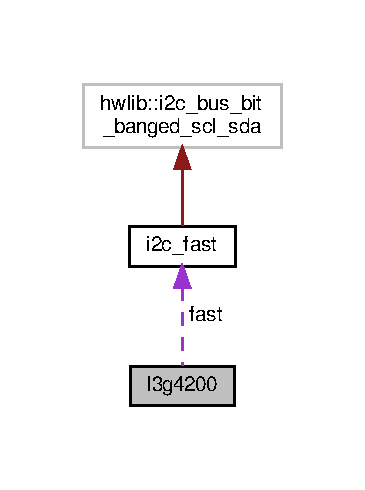
\includegraphics[width=175pt]{classl3g4200__coll__graph}
\end{center}
\end{figure}
\subsection*{Public Member Functions}
\begin{DoxyCompactItemize}
\item 
\hyperlink{classl3g4200_a95f0b60d26992cb2ee03730f38fa3308}{l3g4200} (hwlib\+::i2c\+\_\+bus\+\_\+bit\+\_\+banged\+\_\+scl\+\_\+sda \&bus)
\begin{DoxyCompactList}\small\item\em Constructor of the \hyperlink{classl3g4200}{l3g4200} interface. \end{DoxyCompactList}\item 
\hyperlink{classl3g4200_ada23aa5e15338e522092468a356b728c}{l3g4200} (hwlib\+::i2c\+\_\+bus\+\_\+bit\+\_\+banged\+\_\+scl\+\_\+sda \&bus, uint8\+\_\+t address)
\begin{DoxyCompactList}\small\item\em Constructor of the \hyperlink{classl3g4200}{l3g4200} interface with different address. \end{DoxyCompactList}\item 
void \hyperlink{classl3g4200_a89f0af632b2b19efc614339e479656ed}{reset} ()
\begin{DoxyCompactList}\small\item\em Resets gyro values. \end{DoxyCompactList}\item 
void \hyperlink{classl3g4200_af9dc9bd2b7086a49c1addddce238fcf8}{check\+\_\+status} ()
\begin{DoxyCompactList}\small\item\em Returns when gyroscope data changed. \end{DoxyCompactList}\item 
\mbox{\Hypertarget{classl3g4200_a847c9ae3d63b5f0a46256fdd5d8d0d3b}\label{classl3g4200_a847c9ae3d63b5f0a46256fdd5d8d0d3b}} 
void \hyperlink{classl3g4200_a847c9ae3d63b5f0a46256fdd5d8d0d3b}{set\+\_\+scale} (int scale)
\begin{DoxyCompactList}\small\item\em Changes the gyroscope scale  The gyroscope has different reading modes. With this function you can change these modes to your own liking. You can set the scale 2000, 500 and 250. \end{DoxyCompactList}\item 
void \hyperlink{classl3g4200_affd107a9d8862f7687f1eb3c4fd74ea0}{update} (int interval)
\begin{DoxyCompactList}\small\item\em calculates next gyro values \end{DoxyCompactList}\item 
void \hyperlink{classl3g4200_a9caa7f50a94100706898f049c2bb8d95}{print} ()
\begin{DoxyCompactList}\small\item\em Prints gyro values for demonstration. \end{DoxyCompactList}\item 
void \hyperlink{classl3g4200_a15152a95cc9df7c8e6660c6b62eb48d6}{print\+\_\+dps} ()
\begin{DoxyCompactList}\small\item\em Prints degrees per second values for demonstration. \end{DoxyCompactList}\item 
\mbox{\Hypertarget{classl3g4200_ae9d09120c93a1fefc53606fed017ff7c}\label{classl3g4200_ae9d09120c93a1fefc53606fed017ff7c}} 
void \hyperlink{classl3g4200_ae9d09120c93a1fefc53606fed017ff7c}{wake} ()
\begin{DoxyCompactList}\small\item\em Wakes up the gyroscope. \end{DoxyCompactList}\item 
void \hyperlink{classl3g4200_a2503f466a114e0b31dffe17e486410fd}{sleep} ()
\begin{DoxyCompactList}\small\item\em Tugs in the gyroscope. \end{DoxyCompactList}\item 
void \hyperlink{classl3g4200_a42255bd4a0fc8b465b0b48d9f853ed74}{update\+\_\+temp} ()
\begin{DoxyCompactList}\small\item\em Updates temperature variable. \end{DoxyCompactList}\item 
int \hyperlink{classl3g4200_ad9a37076877d12182d8e259f81fae966}{get\+\_\+temperature} ()
\begin{DoxyCompactList}\small\item\em Gets temperature variable. \end{DoxyCompactList}\item 
int \hyperlink{classl3g4200_a3afab49f43f0224912363175c1560df4}{get\+\_\+x\+\_\+gyro\+\_\+h} ()
\begin{DoxyCompactList}\small\item\em Returns gyro x shifted 8 bits to the right. \end{DoxyCompactList}\item 
int \hyperlink{classl3g4200_a34b780b136282aa2fdace5daeaadb7ac}{get\+\_\+x\+\_\+gyro\+\_\+l} ()
\begin{DoxyCompactList}\small\item\em Returns x gyro variable. \end{DoxyCompactList}\item 
int \hyperlink{classl3g4200_a6c4d995bc9be83ae30d884d0dec95960}{get\+\_\+y\+\_\+gyro\+\_\+h} ()
\begin{DoxyCompactList}\small\item\em Returns y gyro shifted 8 bits to the right. \end{DoxyCompactList}\item 
int \hyperlink{classl3g4200_afb369dc33500b9ef4d32a1f35c066448}{get\+\_\+y\+\_\+gyro\+\_\+l} ()
\begin{DoxyCompactList}\small\item\em Returns y gyro variable. \end{DoxyCompactList}\item 
int \hyperlink{classl3g4200_a48ea66d624cf6147656e65b5ba0e3314}{get\+\_\+z\+\_\+gyro\+\_\+h} ()
\begin{DoxyCompactList}\small\item\em Returns z gyro shifted 8 bits to the right. \end{DoxyCompactList}\item 
int \hyperlink{classl3g4200_a6050692b28be5dd532ed91e346545ca3}{get\+\_\+z\+\_\+gyro\+\_\+l} ()
\begin{DoxyCompactList}\small\item\em Returns z gyro variable. \end{DoxyCompactList}\item 
int \hyperlink{classl3g4200_a5182e240887b44c1178576092a61f5fd}{get\+\_\+dps\+\_\+x\+\_\+h} ()
\begin{DoxyCompactList}\small\item\em Returns x dps shifted 8 bits to the right. \end{DoxyCompactList}\item 
int \hyperlink{classl3g4200_a0c96f1bc6aabb4a5bb4652d3ae703821}{get\+\_\+dps\+\_\+x\+\_\+l} ()
\begin{DoxyCompactList}\small\item\em Returns x dps variable. \end{DoxyCompactList}\item 
int \hyperlink{classl3g4200_a46b55512661be401f9a6b7cb7c87b4a1}{get\+\_\+dps\+\_\+y\+\_\+h} ()
\begin{DoxyCompactList}\small\item\em Returns y dps shifted 8 bits to the right. \end{DoxyCompactList}\item 
int \hyperlink{classl3g4200_adcd400fc92347bad573f020b151e9fb5}{get\+\_\+dps\+\_\+y\+\_\+l} ()
\begin{DoxyCompactList}\small\item\em Returns y dps variable. \end{DoxyCompactList}\item 
int \hyperlink{classl3g4200_ac2b63c3b1af1862adbbe96d4166b3e38}{get\+\_\+dps\+\_\+z\+\_\+h} ()
\begin{DoxyCompactList}\small\item\em Returns z dps shifted 8 bits to the right. \end{DoxyCompactList}\item 
int \hyperlink{classl3g4200_a3ff13048a18eed7c7f03ae50a3bc68bf}{get\+\_\+dps\+\_\+z\+\_\+l} ()
\begin{DoxyCompactList}\small\item\em Returns z dps variable. \end{DoxyCompactList}\end{DoxyCompactItemize}
\subsection*{Public Attributes}
\begin{DoxyCompactItemize}
\item 
\mbox{\Hypertarget{classl3g4200_a85345b78a1d99a87a182e6c93d23fbd8}\label{classl3g4200_a85345b78a1d99a87a182e6c93d23fbd8}} 
\hyperlink{classi2c__fast}{i2c\+\_\+fast} {\bfseries fast} = \{bus, address\}
\end{DoxyCompactItemize}


\subsection{Detailed Description}
interface for \hyperlink{classl3g4200}{l3g4200} 

this class interfaces the \hyperlink{classl3g4200}{l3g4200} chip for the slave arudino and should not be used by the user unless you want to only use one Arudino. 

\subsection{Constructor \& Destructor Documentation}
\mbox{\Hypertarget{classl3g4200_a95f0b60d26992cb2ee03730f38fa3308}\label{classl3g4200_a95f0b60d26992cb2ee03730f38fa3308}} 
\index{l3g4200@{l3g4200}!l3g4200@{l3g4200}}
\index{l3g4200@{l3g4200}!l3g4200@{l3g4200}}
\subsubsection{\texorpdfstring{l3g4200()}{l3g4200()}\hspace{0.1cm}{\footnotesize\ttfamily [1/2]}}
{\footnotesize\ttfamily l3g4200\+::l3g4200 (\begin{DoxyParamCaption}\item[{hwlib\+::i2c\+\_\+bus\+\_\+bit\+\_\+banged\+\_\+scl\+\_\+sda \&}]{bus }\end{DoxyParamCaption})\hspace{0.3cm}{\ttfamily [inline]}}



Constructor of the \hyperlink{classl3g4200}{l3g4200} interface. 

This contructor construct an interface for the \hyperlink{classl3g4200}{l3g4200} chip. \mbox{\Hypertarget{classl3g4200_ada23aa5e15338e522092468a356b728c}\label{classl3g4200_ada23aa5e15338e522092468a356b728c}} 
\index{l3g4200@{l3g4200}!l3g4200@{l3g4200}}
\index{l3g4200@{l3g4200}!l3g4200@{l3g4200}}
\subsubsection{\texorpdfstring{l3g4200()}{l3g4200()}\hspace{0.1cm}{\footnotesize\ttfamily [2/2]}}
{\footnotesize\ttfamily l3g4200\+::l3g4200 (\begin{DoxyParamCaption}\item[{hwlib\+::i2c\+\_\+bus\+\_\+bit\+\_\+banged\+\_\+scl\+\_\+sda \&}]{bus,  }\item[{uint8\+\_\+t}]{address }\end{DoxyParamCaption})\hspace{0.3cm}{\ttfamily [inline]}}



Constructor of the \hyperlink{classl3g4200}{l3g4200} interface with different address. 

This contructor construct an interface for the \hyperlink{classl3g4200}{l3g4200} chip with a diverging address. 

\subsection{Member Function Documentation}
\mbox{\Hypertarget{classl3g4200_af9dc9bd2b7086a49c1addddce238fcf8}\label{classl3g4200_af9dc9bd2b7086a49c1addddce238fcf8}} 
\index{l3g4200@{l3g4200}!check\+\_\+status@{check\+\_\+status}}
\index{check\+\_\+status@{check\+\_\+status}!l3g4200@{l3g4200}}
\subsubsection{\texorpdfstring{check\+\_\+status()}{check\_status()}}
{\footnotesize\ttfamily void l3g4200\+::check\+\_\+status (\begin{DoxyParamCaption}{ }\end{DoxyParamCaption})\hspace{0.3cm}{\ttfamily [inline]}}



Returns when gyroscope data changed. 

This function is used as an stop. The function returns when the gyroscope has written a new value to it\textquotesingle{}s registers. This function made the read data more accurately. \mbox{\Hypertarget{classl3g4200_a5182e240887b44c1178576092a61f5fd}\label{classl3g4200_a5182e240887b44c1178576092a61f5fd}} 
\index{l3g4200@{l3g4200}!get\+\_\+dps\+\_\+x\+\_\+h@{get\+\_\+dps\+\_\+x\+\_\+h}}
\index{get\+\_\+dps\+\_\+x\+\_\+h@{get\+\_\+dps\+\_\+x\+\_\+h}!l3g4200@{l3g4200}}
\subsubsection{\texorpdfstring{get\+\_\+dps\+\_\+x\+\_\+h()}{get\_dps\_x\_h()}}
{\footnotesize\ttfamily int l3g4200\+::get\+\_\+dps\+\_\+x\+\_\+h (\begin{DoxyParamCaption}{ }\end{DoxyParamCaption})\hspace{0.3cm}{\ttfamily [inline]}}



Returns x dps shifted 8 bits to the right. 

This function reads the gyro x variable and returns a the value shifted 8 bits to the right \mbox{\Hypertarget{classl3g4200_a0c96f1bc6aabb4a5bb4652d3ae703821}\label{classl3g4200_a0c96f1bc6aabb4a5bb4652d3ae703821}} 
\index{l3g4200@{l3g4200}!get\+\_\+dps\+\_\+x\+\_\+l@{get\+\_\+dps\+\_\+x\+\_\+l}}
\index{get\+\_\+dps\+\_\+x\+\_\+l@{get\+\_\+dps\+\_\+x\+\_\+l}!l3g4200@{l3g4200}}
\subsubsection{\texorpdfstring{get\+\_\+dps\+\_\+x\+\_\+l()}{get\_dps\_x\_l()}}
{\footnotesize\ttfamily int l3g4200\+::get\+\_\+dps\+\_\+x\+\_\+l (\begin{DoxyParamCaption}{ }\end{DoxyParamCaption})\hspace{0.3cm}{\ttfamily [inline]}}



Returns x dps variable. 

This function returs the x dps variable \mbox{\Hypertarget{classl3g4200_a46b55512661be401f9a6b7cb7c87b4a1}\label{classl3g4200_a46b55512661be401f9a6b7cb7c87b4a1}} 
\index{l3g4200@{l3g4200}!get\+\_\+dps\+\_\+y\+\_\+h@{get\+\_\+dps\+\_\+y\+\_\+h}}
\index{get\+\_\+dps\+\_\+y\+\_\+h@{get\+\_\+dps\+\_\+y\+\_\+h}!l3g4200@{l3g4200}}
\subsubsection{\texorpdfstring{get\+\_\+dps\+\_\+y\+\_\+h()}{get\_dps\_y\_h()}}
{\footnotesize\ttfamily int l3g4200\+::get\+\_\+dps\+\_\+y\+\_\+h (\begin{DoxyParamCaption}{ }\end{DoxyParamCaption})\hspace{0.3cm}{\ttfamily [inline]}}



Returns y dps shifted 8 bits to the right. 

This function reads the gyro x variable and returns a the value shifted 8 bits to the right \mbox{\Hypertarget{classl3g4200_adcd400fc92347bad573f020b151e9fb5}\label{classl3g4200_adcd400fc92347bad573f020b151e9fb5}} 
\index{l3g4200@{l3g4200}!get\+\_\+dps\+\_\+y\+\_\+l@{get\+\_\+dps\+\_\+y\+\_\+l}}
\index{get\+\_\+dps\+\_\+y\+\_\+l@{get\+\_\+dps\+\_\+y\+\_\+l}!l3g4200@{l3g4200}}
\subsubsection{\texorpdfstring{get\+\_\+dps\+\_\+y\+\_\+l()}{get\_dps\_y\_l()}}
{\footnotesize\ttfamily int l3g4200\+::get\+\_\+dps\+\_\+y\+\_\+l (\begin{DoxyParamCaption}{ }\end{DoxyParamCaption})\hspace{0.3cm}{\ttfamily [inline]}}



Returns y dps variable. 

This function returs the y dps variable \mbox{\Hypertarget{classl3g4200_ac2b63c3b1af1862adbbe96d4166b3e38}\label{classl3g4200_ac2b63c3b1af1862adbbe96d4166b3e38}} 
\index{l3g4200@{l3g4200}!get\+\_\+dps\+\_\+z\+\_\+h@{get\+\_\+dps\+\_\+z\+\_\+h}}
\index{get\+\_\+dps\+\_\+z\+\_\+h@{get\+\_\+dps\+\_\+z\+\_\+h}!l3g4200@{l3g4200}}
\subsubsection{\texorpdfstring{get\+\_\+dps\+\_\+z\+\_\+h()}{get\_dps\_z\_h()}}
{\footnotesize\ttfamily int l3g4200\+::get\+\_\+dps\+\_\+z\+\_\+h (\begin{DoxyParamCaption}{ }\end{DoxyParamCaption})\hspace{0.3cm}{\ttfamily [inline]}}



Returns z dps shifted 8 bits to the right. 

This function reads the gyro x variable and returns a the value shifted 8 bits to the right \mbox{\Hypertarget{classl3g4200_a3ff13048a18eed7c7f03ae50a3bc68bf}\label{classl3g4200_a3ff13048a18eed7c7f03ae50a3bc68bf}} 
\index{l3g4200@{l3g4200}!get\+\_\+dps\+\_\+z\+\_\+l@{get\+\_\+dps\+\_\+z\+\_\+l}}
\index{get\+\_\+dps\+\_\+z\+\_\+l@{get\+\_\+dps\+\_\+z\+\_\+l}!l3g4200@{l3g4200}}
\subsubsection{\texorpdfstring{get\+\_\+dps\+\_\+z\+\_\+l()}{get\_dps\_z\_l()}}
{\footnotesize\ttfamily int l3g4200\+::get\+\_\+dps\+\_\+z\+\_\+l (\begin{DoxyParamCaption}{ }\end{DoxyParamCaption})\hspace{0.3cm}{\ttfamily [inline]}}



Returns z dps variable. 

This function returs the z dps variable \mbox{\Hypertarget{classl3g4200_ad9a37076877d12182d8e259f81fae966}\label{classl3g4200_ad9a37076877d12182d8e259f81fae966}} 
\index{l3g4200@{l3g4200}!get\+\_\+temperature@{get\+\_\+temperature}}
\index{get\+\_\+temperature@{get\+\_\+temperature}!l3g4200@{l3g4200}}
\subsubsection{\texorpdfstring{get\+\_\+temperature()}{get\_temperature()}}
{\footnotesize\ttfamily int l3g4200\+::get\+\_\+temperature (\begin{DoxyParamCaption}{ }\end{DoxyParamCaption})\hspace{0.3cm}{\ttfamily [inline]}}



Gets temperature variable. 

This function returns the temperature value \mbox{\Hypertarget{classl3g4200_a3afab49f43f0224912363175c1560df4}\label{classl3g4200_a3afab49f43f0224912363175c1560df4}} 
\index{l3g4200@{l3g4200}!get\+\_\+x\+\_\+gyro\+\_\+h@{get\+\_\+x\+\_\+gyro\+\_\+h}}
\index{get\+\_\+x\+\_\+gyro\+\_\+h@{get\+\_\+x\+\_\+gyro\+\_\+h}!l3g4200@{l3g4200}}
\subsubsection{\texorpdfstring{get\+\_\+x\+\_\+gyro\+\_\+h()}{get\_x\_gyro\_h()}}
{\footnotesize\ttfamily int l3g4200\+::get\+\_\+x\+\_\+gyro\+\_\+h (\begin{DoxyParamCaption}{ }\end{DoxyParamCaption})\hspace{0.3cm}{\ttfamily [inline]}}



Returns gyro x shifted 8 bits to the right. 

This function reads the gyro x variable and returns a the value shifted 8 bits to the right \mbox{\Hypertarget{classl3g4200_a34b780b136282aa2fdace5daeaadb7ac}\label{classl3g4200_a34b780b136282aa2fdace5daeaadb7ac}} 
\index{l3g4200@{l3g4200}!get\+\_\+x\+\_\+gyro\+\_\+l@{get\+\_\+x\+\_\+gyro\+\_\+l}}
\index{get\+\_\+x\+\_\+gyro\+\_\+l@{get\+\_\+x\+\_\+gyro\+\_\+l}!l3g4200@{l3g4200}}
\subsubsection{\texorpdfstring{get\+\_\+x\+\_\+gyro\+\_\+l()}{get\_x\_gyro\_l()}}
{\footnotesize\ttfamily int l3g4200\+::get\+\_\+x\+\_\+gyro\+\_\+l (\begin{DoxyParamCaption}{ }\end{DoxyParamCaption})\hspace{0.3cm}{\ttfamily [inline]}}



Returns x gyro variable. 

This function returs the x gyro variable \mbox{\Hypertarget{classl3g4200_a6c4d995bc9be83ae30d884d0dec95960}\label{classl3g4200_a6c4d995bc9be83ae30d884d0dec95960}} 
\index{l3g4200@{l3g4200}!get\+\_\+y\+\_\+gyro\+\_\+h@{get\+\_\+y\+\_\+gyro\+\_\+h}}
\index{get\+\_\+y\+\_\+gyro\+\_\+h@{get\+\_\+y\+\_\+gyro\+\_\+h}!l3g4200@{l3g4200}}
\subsubsection{\texorpdfstring{get\+\_\+y\+\_\+gyro\+\_\+h()}{get\_y\_gyro\_h()}}
{\footnotesize\ttfamily int l3g4200\+::get\+\_\+y\+\_\+gyro\+\_\+h (\begin{DoxyParamCaption}{ }\end{DoxyParamCaption})\hspace{0.3cm}{\ttfamily [inline]}}



Returns y gyro shifted 8 bits to the right. 

This function reads the gyro x variable and returns a the value shifted 8 bits to the right \mbox{\Hypertarget{classl3g4200_afb369dc33500b9ef4d32a1f35c066448}\label{classl3g4200_afb369dc33500b9ef4d32a1f35c066448}} 
\index{l3g4200@{l3g4200}!get\+\_\+y\+\_\+gyro\+\_\+l@{get\+\_\+y\+\_\+gyro\+\_\+l}}
\index{get\+\_\+y\+\_\+gyro\+\_\+l@{get\+\_\+y\+\_\+gyro\+\_\+l}!l3g4200@{l3g4200}}
\subsubsection{\texorpdfstring{get\+\_\+y\+\_\+gyro\+\_\+l()}{get\_y\_gyro\_l()}}
{\footnotesize\ttfamily int l3g4200\+::get\+\_\+y\+\_\+gyro\+\_\+l (\begin{DoxyParamCaption}{ }\end{DoxyParamCaption})\hspace{0.3cm}{\ttfamily [inline]}}



Returns y gyro variable. 

This function returs the y gyro variable \mbox{\Hypertarget{classl3g4200_a48ea66d624cf6147656e65b5ba0e3314}\label{classl3g4200_a48ea66d624cf6147656e65b5ba0e3314}} 
\index{l3g4200@{l3g4200}!get\+\_\+z\+\_\+gyro\+\_\+h@{get\+\_\+z\+\_\+gyro\+\_\+h}}
\index{get\+\_\+z\+\_\+gyro\+\_\+h@{get\+\_\+z\+\_\+gyro\+\_\+h}!l3g4200@{l3g4200}}
\subsubsection{\texorpdfstring{get\+\_\+z\+\_\+gyro\+\_\+h()}{get\_z\_gyro\_h()}}
{\footnotesize\ttfamily int l3g4200\+::get\+\_\+z\+\_\+gyro\+\_\+h (\begin{DoxyParamCaption}{ }\end{DoxyParamCaption})\hspace{0.3cm}{\ttfamily [inline]}}



Returns z gyro shifted 8 bits to the right. 

This function reads the gyro x variable and returns a the value shifted 8 bits to the right \mbox{\Hypertarget{classl3g4200_a6050692b28be5dd532ed91e346545ca3}\label{classl3g4200_a6050692b28be5dd532ed91e346545ca3}} 
\index{l3g4200@{l3g4200}!get\+\_\+z\+\_\+gyro\+\_\+l@{get\+\_\+z\+\_\+gyro\+\_\+l}}
\index{get\+\_\+z\+\_\+gyro\+\_\+l@{get\+\_\+z\+\_\+gyro\+\_\+l}!l3g4200@{l3g4200}}
\subsubsection{\texorpdfstring{get\+\_\+z\+\_\+gyro\+\_\+l()}{get\_z\_gyro\_l()}}
{\footnotesize\ttfamily int l3g4200\+::get\+\_\+z\+\_\+gyro\+\_\+l (\begin{DoxyParamCaption}{ }\end{DoxyParamCaption})\hspace{0.3cm}{\ttfamily [inline]}}



Returns z gyro variable. 

This function returs the z gyro variable \mbox{\Hypertarget{classl3g4200_a9caa7f50a94100706898f049c2bb8d95}\label{classl3g4200_a9caa7f50a94100706898f049c2bb8d95}} 
\index{l3g4200@{l3g4200}!print@{print}}
\index{print@{print}!l3g4200@{l3g4200}}
\subsubsection{\texorpdfstring{print()}{print()}}
{\footnotesize\ttfamily void l3g4200\+::print (\begin{DoxyParamCaption}{ }\end{DoxyParamCaption})\hspace{0.3cm}{\ttfamily [inline]}}



Prints gyro values for demonstration. 

This function prints the gyro values for the demonstration and can be used for debugging. \mbox{\Hypertarget{classl3g4200_a15152a95cc9df7c8e6660c6b62eb48d6}\label{classl3g4200_a15152a95cc9df7c8e6660c6b62eb48d6}} 
\index{l3g4200@{l3g4200}!print\+\_\+dps@{print\+\_\+dps}}
\index{print\+\_\+dps@{print\+\_\+dps}!l3g4200@{l3g4200}}
\subsubsection{\texorpdfstring{print\+\_\+dps()}{print\_dps()}}
{\footnotesize\ttfamily void l3g4200\+::print\+\_\+dps (\begin{DoxyParamCaption}{ }\end{DoxyParamCaption})\hspace{0.3cm}{\ttfamily [inline]}}



Prints degrees per second values for demonstration. 

This function prints the degrees per second values for the demonstration and can be used for debugging. \mbox{\Hypertarget{classl3g4200_a89f0af632b2b19efc614339e479656ed}\label{classl3g4200_a89f0af632b2b19efc614339e479656ed}} 
\index{l3g4200@{l3g4200}!reset@{reset}}
\index{reset@{reset}!l3g4200@{l3g4200}}
\subsubsection{\texorpdfstring{reset()}{reset()}}
{\footnotesize\ttfamily void l3g4200\+::reset (\begin{DoxyParamCaption}{ }\end{DoxyParamCaption})\hspace{0.3cm}{\ttfamily [inline]}}



Resets gyro values. 

This function resets all gyro values to zero. \mbox{\Hypertarget{classl3g4200_a2503f466a114e0b31dffe17e486410fd}\label{classl3g4200_a2503f466a114e0b31dffe17e486410fd}} 
\index{l3g4200@{l3g4200}!sleep@{sleep}}
\index{sleep@{sleep}!l3g4200@{l3g4200}}
\subsubsection{\texorpdfstring{sleep()}{sleep()}}
{\footnotesize\ttfamily void l3g4200\+::sleep (\begin{DoxyParamCaption}{ }\end{DoxyParamCaption})\hspace{0.3cm}{\ttfamily [inline]}}



Tugs in the gyroscope. 

This function sends a bit to the sleep register of the \hyperlink{classl3g4200}{l3g4200} and turns it into sleepmode \mbox{\Hypertarget{classl3g4200_affd107a9d8862f7687f1eb3c4fd74ea0}\label{classl3g4200_affd107a9d8862f7687f1eb3c4fd74ea0}} 
\index{l3g4200@{l3g4200}!update@{update}}
\index{update@{update}!l3g4200@{l3g4200}}
\subsubsection{\texorpdfstring{update()}{update()}}
{\footnotesize\ttfamily void l3g4200\+::update (\begin{DoxyParamCaption}\item[{int}]{interval }\end{DoxyParamCaption})\hspace{0.3cm}{\ttfamily [inline]}}



calculates next gyro values 

This function updates all the gyro values and also generates the next value of the gyro based on the degree per second values read out of the \hyperlink{classl3g4200}{l3g4200} registers. \mbox{\Hypertarget{classl3g4200_a42255bd4a0fc8b465b0b48d9f853ed74}\label{classl3g4200_a42255bd4a0fc8b465b0b48d9f853ed74}} 
\index{l3g4200@{l3g4200}!update\+\_\+temp@{update\+\_\+temp}}
\index{update\+\_\+temp@{update\+\_\+temp}!l3g4200@{l3g4200}}
\subsubsection{\texorpdfstring{update\+\_\+temp()}{update\_temp()}}
{\footnotesize\ttfamily void l3g4200\+::update\+\_\+temp (\begin{DoxyParamCaption}{ }\end{DoxyParamCaption})\hspace{0.3cm}{\ttfamily [inline]}}



Updates temperature variable. 

This function updates the temperature variable by reading the temperature register on the \hyperlink{classl3g4200}{l3g4200} 

The documentation for this class was generated from the following file\+:\begin{DoxyCompactItemize}
\item 
src/\+Sogyrolib/\+Slave/\hyperlink{l3g4200_8hpp}{l3g4200.\+hpp}\end{DoxyCompactItemize}

\hypertarget{classslave}{}\section{slave Class Reference}
\label{classslave}\index{slave@{slave}}


Class to create a S\+PI slave for Arduino.  




{\ttfamily \#include $<$slave.\+hpp$>$}

\subsection*{Public Member Functions}
\begin{DoxyCompactItemize}
\item 
\mbox{\Hypertarget{classslave_af73020d7757901f0c58619b2abb6bb44}\label{classslave_af73020d7757901f0c58619b2abb6bb44}} 
{\bfseries slave} (\hyperlink{classl3g4200}{l3g4200} \&gyro)
\item 
void \hyperlink{classslave_ad7387f369836c10790362781d5ce92da}{byte\+\_\+send} ()
\begin{DoxyCompactList}\small\item\em Sends byte to master. \end{DoxyCompactList}\item 
void \hyperlink{classslave_af42612432810eefab015f40c32958fe9}{byte\+\_\+read} ()
\begin{DoxyCompactList}\small\item\em Reads byte from master. \end{DoxyCompactList}\item 
void \hyperlink{classslave_a47169cdf6f0aaa0c303c5d860c89bef2}{print} ()
\begin{DoxyCompactList}\small\item\em Prints incomming byte. \end{DoxyCompactList}\item 
void \hyperlink{classslave_ab93bbc9a1b5e8b5fafb01b63e05440b0}{check} ()
\begin{DoxyCompactList}\small\item\em Checks incomming byte to execute gyroscope function. \end{DoxyCompactList}\end{DoxyCompactItemize}
\subsection*{Public Attributes}
\begin{DoxyCompactItemize}
\item 
\mbox{\Hypertarget{classslave_af3671b4d8f443e427a0610ad2a2f2977}\label{classslave_af3671b4d8f443e427a0610ad2a2f2977}} 
uint\+\_\+fast8\+\_\+t {\bfseries data\+\_\+in} = 0x0
\item 
\mbox{\Hypertarget{classslave_a737d2cc1027a4344b862a15bafbf7e81}\label{classslave_a737d2cc1027a4344b862a15bafbf7e81}} 
uint\+\_\+fast8\+\_\+t {\bfseries data\+\_\+out} = 0x68
\item 
\mbox{\Hypertarget{classslave_a1df63e87edf58a2c29c3c42b1562d1d0}\label{classslave_a1df63e87edf58a2c29c3c42b1562d1d0}} 
int {\bfseries position} = 0
\end{DoxyCompactItemize}


\subsection{Detailed Description}
Class to create a S\+PI slave for Arduino. 

This class is used to make a S\+PI bus slave to connect multiple Arduino\textquotesingle{}s with each other. 

\subsection{Member Function Documentation}
\mbox{\Hypertarget{classslave_af42612432810eefab015f40c32958fe9}\label{classslave_af42612432810eefab015f40c32958fe9}} 
\index{slave@{slave}!byte\+\_\+read@{byte\+\_\+read}}
\index{byte\+\_\+read@{byte\+\_\+read}!slave@{slave}}
\subsubsection{\texorpdfstring{byte\+\_\+read()}{byte\_read()}}
{\footnotesize\ttfamily void slave\+::byte\+\_\+read (\begin{DoxyParamCaption}{ }\end{DoxyParamCaption})\hspace{0.3cm}{\ttfamily [inline]}}



Reads byte from master. 

This function reads the incomming byte from the master Arduino. \mbox{\Hypertarget{classslave_ad7387f369836c10790362781d5ce92da}\label{classslave_ad7387f369836c10790362781d5ce92da}} 
\index{slave@{slave}!byte\+\_\+send@{byte\+\_\+send}}
\index{byte\+\_\+send@{byte\+\_\+send}!slave@{slave}}
\subsubsection{\texorpdfstring{byte\+\_\+send()}{byte\_send()}}
{\footnotesize\ttfamily void slave\+::byte\+\_\+send (\begin{DoxyParamCaption}{ }\end{DoxyParamCaption})\hspace{0.3cm}{\ttfamily [inline]}}



Sends byte to master. 

This function writes a byte to the master Arduino \mbox{\Hypertarget{classslave_ab93bbc9a1b5e8b5fafb01b63e05440b0}\label{classslave_ab93bbc9a1b5e8b5fafb01b63e05440b0}} 
\index{slave@{slave}!check@{check}}
\index{check@{check}!slave@{slave}}
\subsubsection{\texorpdfstring{check()}{check()}}
{\footnotesize\ttfamily void slave\+::check (\begin{DoxyParamCaption}{ }\end{DoxyParamCaption})\hspace{0.3cm}{\ttfamily [inline]}}



Checks incomming byte to execute gyroscope function. 

This function checks the incomming byte and determines wich function of the gyroscope library it schould execute. \mbox{\Hypertarget{classslave_a47169cdf6f0aaa0c303c5d860c89bef2}\label{classslave_a47169cdf6f0aaa0c303c5d860c89bef2}} 
\index{slave@{slave}!print@{print}}
\index{print@{print}!slave@{slave}}
\subsubsection{\texorpdfstring{print()}{print()}}
{\footnotesize\ttfamily void slave\+::print (\begin{DoxyParamCaption}{ }\end{DoxyParamCaption})\hspace{0.3cm}{\ttfamily [inline]}}



Prints incomming byte. 

This function prints the incomming byte buffer 

The documentation for this class was generated from the following file\+:\begin{DoxyCompactItemize}
\item 
src/\+Sogyrolib/\+Slave/\hyperlink{slave_8hpp}{slave.\+hpp}\end{DoxyCompactItemize}

\hypertarget{classsogyro}{}\section{sogyro Class Reference}
\label{classsogyro}\index{sogyro@{sogyro}}


Class that interfaces the arduino connected to a gyro scope.  




{\ttfamily \#include $<$l3g4\+\_\+master.\+hpp$>$}



Inheritance diagram for sogyro\+:
\nopagebreak
\begin{figure}[H]
\begin{center}
\leavevmode
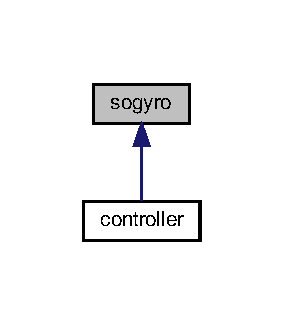
\includegraphics[width=136pt]{classsogyro__inherit__graph}
\end{center}
\end{figure}
\subsection*{Public Member Functions}
\begin{DoxyCompactItemize}
\item 
\hyperlink{classsogyro_ac7d4d6dd2fb21e10e9ad95262520635b}{sogyro} (hwlib\+::spi\+\_\+bus\+\_\+bit\+\_\+banged\+\_\+sclk\+\_\+mosi\+\_\+miso \&bus, hwlib\+::target\+::pin\+\_\+out \&cs)
\begin{DoxyCompactList}\small\item\em Constructs an interface for the Slave Arduino Nano. \end{DoxyCompactList}\item 
\hyperlink{classsogyro_a43e6a4ab150faccd436e63c9f41c885d}{sogyro} (hwlib\+::spi\+\_\+bus\+\_\+bit\+\_\+banged\+\_\+sclk\+\_\+mosi\+\_\+miso \&bus, hwlib\+::target\+::pin\+\_\+out \&cs, int mode)
\begin{DoxyCompactList}\small\item\em Constructs an interface for the Slave Arduino Nano. \end{DoxyCompactList}\item 
int \hyperlink{classsogyro_ae8d4d35c21a057146898ee56ccbfca70}{fast\+\_\+read} (uint8\+\_\+t address)
\begin{DoxyCompactList}\small\item\em function to read and write data. \end{DoxyCompactList}\item 
int \hyperlink{classsogyro_a65a601a9536aefcad18969ef5969fe11}{fast\+\_\+read} (uint8\+\_\+t high, uint8\+\_\+t low)
\begin{DoxyCompactList}\small\item\em function to read and write data. \end{DoxyCompactList}\item 
int \hyperlink{classsogyro_a69d818342aa6a4688afc26d8db62af33}{get\+\_\+gyro\+\_\+x} ()
\begin{DoxyCompactList}\small\item\em Returns gyro x axis data in degrees. \end{DoxyCompactList}\item 
int \hyperlink{classsogyro_a5d0a23dd18a82284625c479df3d1bb9b}{get\+\_\+gyro\+\_\+y} ()
\begin{DoxyCompactList}\small\item\em Returns gyro y axis data in degrees. \end{DoxyCompactList}\item 
int \hyperlink{classsogyro_a71e8f90b8fcb6a3351600a1dda5c8923}{get\+\_\+gyro\+\_\+z} ()
\begin{DoxyCompactList}\small\item\em Returns gyro z axis data in degrees. \end{DoxyCompactList}\item 
int \hyperlink{classsogyro_acad639f73b31704bd60dcb81ca4d8ed1}{get\+\_\+dps\+\_\+x} ()
\begin{DoxyCompactList}\small\item\em Returns gyro x dps data in degrees per second. \end{DoxyCompactList}\item 
int \hyperlink{classsogyro_add0d7fc633b0410127e243f2eba19f2d}{get\+\_\+dps\+\_\+y} ()
\begin{DoxyCompactList}\small\item\em Returns gyro y dps data in degrees per second. \end{DoxyCompactList}\item 
int \hyperlink{classsogyro_acaaac40f021d89a77c093b2303e6e79c}{get\+\_\+dps\+\_\+z} ()
\begin{DoxyCompactList}\small\item\em Returns gyro z dps data in degrees per second. \end{DoxyCompactList}\item 
int \hyperlink{classsogyro_a762e79e3874507ba58910d90a115ea70}{get\+\_\+temp} ()
\begin{DoxyCompactList}\small\item\em Returns temprature data in degrees. \end{DoxyCompactList}\item 
\mbox{\Hypertarget{classsogyro_ac253f3fa45e48f2f31a6211bb5c60894}\label{classsogyro_ac253f3fa45e48f2f31a6211bb5c60894}} 
void \hyperlink{classsogyro_ac253f3fa45e48f2f31a6211bb5c60894}{set\+\_\+scale} (int scale)
\begin{DoxyCompactList}\small\item\em Changes the scale of the gyroscope  This function is used to change the gyroscope scale to either 250, 500 or 2000. \end{DoxyCompactList}\item 
\mbox{\Hypertarget{classsogyro_a8a0a938e79e5ab36803c4922fe88bbcb}\label{classsogyro_a8a0a938e79e5ab36803c4922fe88bbcb}} 
int \hyperlink{classsogyro_a8a0a938e79e5ab36803c4922fe88bbcb}{wake} ()
\begin{DoxyCompactList}\small\item\em Wakes up the gyroscope  This function is used to wakes up the gyroscope from sleep mode. \end{DoxyCompactList}\item 
\mbox{\Hypertarget{classsogyro_a8f4d69c173d5552e22ce9e79bca19d3f}\label{classsogyro_a8f4d69c173d5552e22ce9e79bca19d3f}} 
int \hyperlink{classsogyro_a8f4d69c173d5552e22ce9e79bca19d3f}{sleep} ()
\begin{DoxyCompactList}\small\item\em Tugs in the gyroscope  This function is used to to set the gyroscope to sleep mode. \end{DoxyCompactList}\item 
\mbox{\Hypertarget{classsogyro_a8c5d413a3026f0a80fb7929617349686}\label{classsogyro_a8c5d413a3026f0a80fb7929617349686}} 
void {\bfseries reset} ()
\end{DoxyCompactItemize}


\subsection{Detailed Description}
Class that interfaces the arduino connected to a gyro scope. 

A class that interfaces the Slave Arduino Nano through a spi bus that is dedicated only to the Arduino Nano. The Arduino Nano is connected to a L3\+G4200 gyroscope. The functions of this class send register adresses to the Arduino Nano and then Arduino Nano returns the correpsonding data. 

\subsection{Constructor \& Destructor Documentation}
\mbox{\Hypertarget{classsogyro_ac7d4d6dd2fb21e10e9ad95262520635b}\label{classsogyro_ac7d4d6dd2fb21e10e9ad95262520635b}} 
\index{sogyro@{sogyro}!sogyro@{sogyro}}
\index{sogyro@{sogyro}!sogyro@{sogyro}}
\subsubsection{\texorpdfstring{sogyro()}{sogyro()}\hspace{0.1cm}{\footnotesize\ttfamily [1/2]}}
{\footnotesize\ttfamily sogyro\+::sogyro (\begin{DoxyParamCaption}\item[{hwlib\+::spi\+\_\+bus\+\_\+bit\+\_\+banged\+\_\+sclk\+\_\+mosi\+\_\+miso \&}]{bus,  }\item[{hwlib\+::target\+::pin\+\_\+out \&}]{cs }\end{DoxyParamCaption})\hspace{0.3cm}{\ttfamily [inline]}}



Constructs an interface for the Slave Arduino Nano. 

This constructor creates an interface for the Slave Arduino Nano using a spi bus and a enabler pin. \mbox{\Hypertarget{classsogyro_a43e6a4ab150faccd436e63c9f41c885d}\label{classsogyro_a43e6a4ab150faccd436e63c9f41c885d}} 
\index{sogyro@{sogyro}!sogyro@{sogyro}}
\index{sogyro@{sogyro}!sogyro@{sogyro}}
\subsubsection{\texorpdfstring{sogyro()}{sogyro()}\hspace{0.1cm}{\footnotesize\ttfamily [2/2]}}
{\footnotesize\ttfamily sogyro\+::sogyro (\begin{DoxyParamCaption}\item[{hwlib\+::spi\+\_\+bus\+\_\+bit\+\_\+banged\+\_\+sclk\+\_\+mosi\+\_\+miso \&}]{bus,  }\item[{hwlib\+::target\+::pin\+\_\+out \&}]{cs,  }\item[{int}]{mode }\end{DoxyParamCaption})\hspace{0.3cm}{\ttfamily [inline]}}



Constructs an interface for the Slave Arduino Nano. 

This constructor creates an interface for the Slave Arduino Nano using a spi bus and a enabler pin and also sets the scale for the gyroscope. 

\subsection{Member Function Documentation}
\mbox{\Hypertarget{classsogyro_ae8d4d35c21a057146898ee56ccbfca70}\label{classsogyro_ae8d4d35c21a057146898ee56ccbfca70}} 
\index{sogyro@{sogyro}!fast\+\_\+read@{fast\+\_\+read}}
\index{fast\+\_\+read@{fast\+\_\+read}!sogyro@{sogyro}}
\subsubsection{\texorpdfstring{fast\+\_\+read()}{fast\_read()}\hspace{0.1cm}{\footnotesize\ttfamily [1/2]}}
{\footnotesize\ttfamily int sogyro\+::fast\+\_\+read (\begin{DoxyParamCaption}\item[{uint8\+\_\+t}]{address }\end{DoxyParamCaption})\hspace{0.3cm}{\ttfamily [inline]}}



function to read and write data. 

A function used to write 1 byte of data to read 1 byte of data. \mbox{\Hypertarget{classsogyro_a65a601a9536aefcad18969ef5969fe11}\label{classsogyro_a65a601a9536aefcad18969ef5969fe11}} 
\index{sogyro@{sogyro}!fast\+\_\+read@{fast\+\_\+read}}
\index{fast\+\_\+read@{fast\+\_\+read}!sogyro@{sogyro}}
\subsubsection{\texorpdfstring{fast\+\_\+read()}{fast\_read()}\hspace{0.1cm}{\footnotesize\ttfamily [2/2]}}
{\footnotesize\ttfamily int sogyro\+::fast\+\_\+read (\begin{DoxyParamCaption}\item[{uint8\+\_\+t}]{high,  }\item[{uint8\+\_\+t}]{low }\end{DoxyParamCaption})\hspace{0.3cm}{\ttfamily [inline]}}



function to read and write data. 

A function used to write 2 byte of data to read 2 bytes of data. The function merges the to bytes of data and then return them as an uint16\+\_\+t value. \mbox{\Hypertarget{classsogyro_acad639f73b31704bd60dcb81ca4d8ed1}\label{classsogyro_acad639f73b31704bd60dcb81ca4d8ed1}} 
\index{sogyro@{sogyro}!get\+\_\+dps\+\_\+x@{get\+\_\+dps\+\_\+x}}
\index{get\+\_\+dps\+\_\+x@{get\+\_\+dps\+\_\+x}!sogyro@{sogyro}}
\subsubsection{\texorpdfstring{get\+\_\+dps\+\_\+x()}{get\_dps\_x()}}
{\footnotesize\ttfamily int sogyro\+::get\+\_\+dps\+\_\+x (\begin{DoxyParamCaption}{ }\end{DoxyParamCaption})\hspace{0.3cm}{\ttfamily [inline]}}



Returns gyro x dps data in degrees per second. 

This function is used to recieve the current degrees per second x value from the slave Arduino Nano. \mbox{\Hypertarget{classsogyro_add0d7fc633b0410127e243f2eba19f2d}\label{classsogyro_add0d7fc633b0410127e243f2eba19f2d}} 
\index{sogyro@{sogyro}!get\+\_\+dps\+\_\+y@{get\+\_\+dps\+\_\+y}}
\index{get\+\_\+dps\+\_\+y@{get\+\_\+dps\+\_\+y}!sogyro@{sogyro}}
\subsubsection{\texorpdfstring{get\+\_\+dps\+\_\+y()}{get\_dps\_y()}}
{\footnotesize\ttfamily int sogyro\+::get\+\_\+dps\+\_\+y (\begin{DoxyParamCaption}{ }\end{DoxyParamCaption})\hspace{0.3cm}{\ttfamily [inline]}}



Returns gyro y dps data in degrees per second. 

This function is used to recieve the current degrees per second y value from the slave Arduino Nano. \mbox{\Hypertarget{classsogyro_acaaac40f021d89a77c093b2303e6e79c}\label{classsogyro_acaaac40f021d89a77c093b2303e6e79c}} 
\index{sogyro@{sogyro}!get\+\_\+dps\+\_\+z@{get\+\_\+dps\+\_\+z}}
\index{get\+\_\+dps\+\_\+z@{get\+\_\+dps\+\_\+z}!sogyro@{sogyro}}
\subsubsection{\texorpdfstring{get\+\_\+dps\+\_\+z()}{get\_dps\_z()}}
{\footnotesize\ttfamily int sogyro\+::get\+\_\+dps\+\_\+z (\begin{DoxyParamCaption}{ }\end{DoxyParamCaption})\hspace{0.3cm}{\ttfamily [inline]}}



Returns gyro z dps data in degrees per second. 

This function is used to recieve the current degrees per second z value from the slave Arduino Nano. \mbox{\Hypertarget{classsogyro_a69d818342aa6a4688afc26d8db62af33}\label{classsogyro_a69d818342aa6a4688afc26d8db62af33}} 
\index{sogyro@{sogyro}!get\+\_\+gyro\+\_\+x@{get\+\_\+gyro\+\_\+x}}
\index{get\+\_\+gyro\+\_\+x@{get\+\_\+gyro\+\_\+x}!sogyro@{sogyro}}
\subsubsection{\texorpdfstring{get\+\_\+gyro\+\_\+x()}{get\_gyro\_x()}}
{\footnotesize\ttfamily int sogyro\+::get\+\_\+gyro\+\_\+x (\begin{DoxyParamCaption}{ }\end{DoxyParamCaption})\hspace{0.3cm}{\ttfamily [inline]}}



Returns gyro x axis data in degrees. 

This function is used to recieve the current gyro x axis from the slave Arduino Nano \mbox{\Hypertarget{classsogyro_a5d0a23dd18a82284625c479df3d1bb9b}\label{classsogyro_a5d0a23dd18a82284625c479df3d1bb9b}} 
\index{sogyro@{sogyro}!get\+\_\+gyro\+\_\+y@{get\+\_\+gyro\+\_\+y}}
\index{get\+\_\+gyro\+\_\+y@{get\+\_\+gyro\+\_\+y}!sogyro@{sogyro}}
\subsubsection{\texorpdfstring{get\+\_\+gyro\+\_\+y()}{get\_gyro\_y()}}
{\footnotesize\ttfamily int sogyro\+::get\+\_\+gyro\+\_\+y (\begin{DoxyParamCaption}{ }\end{DoxyParamCaption})\hspace{0.3cm}{\ttfamily [inline]}}



Returns gyro y axis data in degrees. 

This function is used to recieve the current gyro y axis from the slave Arduino Nano \mbox{\Hypertarget{classsogyro_a71e8f90b8fcb6a3351600a1dda5c8923}\label{classsogyro_a71e8f90b8fcb6a3351600a1dda5c8923}} 
\index{sogyro@{sogyro}!get\+\_\+gyro\+\_\+z@{get\+\_\+gyro\+\_\+z}}
\index{get\+\_\+gyro\+\_\+z@{get\+\_\+gyro\+\_\+z}!sogyro@{sogyro}}
\subsubsection{\texorpdfstring{get\+\_\+gyro\+\_\+z()}{get\_gyro\_z()}}
{\footnotesize\ttfamily int sogyro\+::get\+\_\+gyro\+\_\+z (\begin{DoxyParamCaption}{ }\end{DoxyParamCaption})\hspace{0.3cm}{\ttfamily [inline]}}



Returns gyro z axis data in degrees. 

This function is used to recieve the current gyro z axis from the slave Arduino Nano \mbox{\Hypertarget{classsogyro_a762e79e3874507ba58910d90a115ea70}\label{classsogyro_a762e79e3874507ba58910d90a115ea70}} 
\index{sogyro@{sogyro}!get\+\_\+temp@{get\+\_\+temp}}
\index{get\+\_\+temp@{get\+\_\+temp}!sogyro@{sogyro}}
\subsubsection{\texorpdfstring{get\+\_\+temp()}{get\_temp()}}
{\footnotesize\ttfamily int sogyro\+::get\+\_\+temp (\begin{DoxyParamCaption}{ }\end{DoxyParamCaption})\hspace{0.3cm}{\ttfamily [inline]}}



Returns temprature data in degrees. 

This function is used to recieve the current temprature from the slave Arduino Nano. 

The documentation for this class was generated from the following file\+:\begin{DoxyCompactItemize}
\item 
src/\+Sogyrolib/\+Master/\hyperlink{l3g4__master_8hpp}{l3g4\+\_\+master.\+hpp}\end{DoxyCompactItemize}

\chapter{File Documentation}
\hypertarget{controller_8hpp}{}\section{src/\+Sogyrolib/\+Master/controller.hpp File Reference}
\label{controller_8hpp}\index{src/\+Sogyrolib/\+Master/controller.\+hpp@{src/\+Sogyrolib/\+Master/controller.\+hpp}}
{\ttfamily \#include \char`\"{}l3g4\+\_\+master.\+hpp\char`\"{}}\newline
Include dependency graph for controller.\+hpp\+:
\nopagebreak
\begin{figure}[H]
\begin{center}
\leavevmode
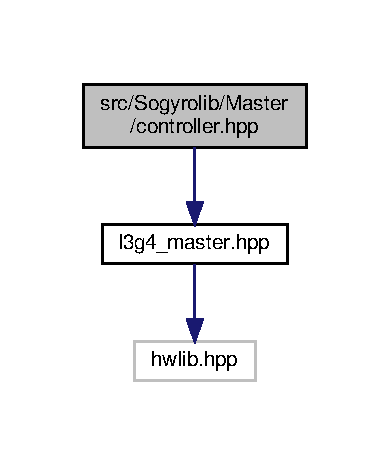
\includegraphics[width=187pt]{controller_8hpp__incl}
\end{center}
\end{figure}
\subsection*{Classes}
\begin{DoxyCompactItemize}
\item 
class \hyperlink{classcontroller}{controller}
\begin{DoxyCompactList}\small\item\em Gyroscope decorator. \end{DoxyCompactList}\end{DoxyCompactItemize}

\hypertarget{l3g4__master_8hpp}{}\section{src/\+Sogyrolib/\+Master/l3g4\+\_\+master.hpp File Reference}
\label{l3g4__master_8hpp}\index{src/\+Sogyrolib/\+Master/l3g4\+\_\+master.\+hpp@{src/\+Sogyrolib/\+Master/l3g4\+\_\+master.\+hpp}}
{\ttfamily \#include \char`\"{}hwlib.\+hpp\char`\"{}}\newline
Include dependency graph for l3g4\+\_\+master.\+hpp\+:
\nopagebreak
\begin{figure}[H]
\begin{center}
\leavevmode
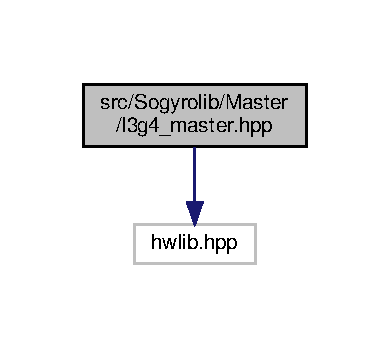
\includegraphics[width=187pt]{l3g4__master_8hpp__incl}
\end{center}
\end{figure}
This graph shows which files directly or indirectly include this file\+:
\nopagebreak
\begin{figure}[H]
\begin{center}
\leavevmode
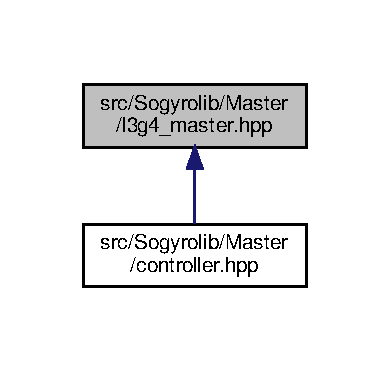
\includegraphics[width=187pt]{l3g4__master_8hpp__dep__incl}
\end{center}
\end{figure}
\subsection*{Classes}
\begin{DoxyCompactItemize}
\item 
class \hyperlink{classsogyro}{sogyro}
\begin{DoxyCompactList}\small\item\em Class that interfaces the arduino connected to a gyro scope. \end{DoxyCompactList}\end{DoxyCompactItemize}

\hypertarget{i2c__fast_8hpp}{}\section{src/\+Sogyrolib/\+Slave/i2c\+\_\+fast.hpp File Reference}
\label{i2c__fast_8hpp}\index{src/\+Sogyrolib/\+Slave/i2c\+\_\+fast.\+hpp@{src/\+Sogyrolib/\+Slave/i2c\+\_\+fast.\+hpp}}
{\ttfamily \#include \char`\"{}hwlib.\+hpp\char`\"{}}\newline
Include dependency graph for i2c\+\_\+fast.\+hpp\+:
\nopagebreak
\begin{figure}[H]
\begin{center}
\leavevmode
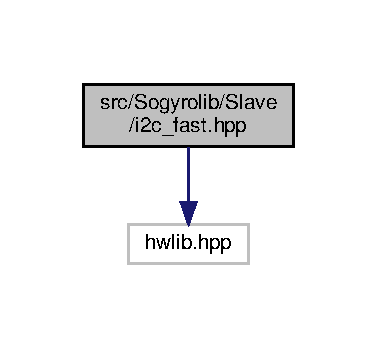
\includegraphics[width=181pt]{i2c__fast_8hpp__incl}
\end{center}
\end{figure}
This graph shows which files directly or indirectly include this file\+:
\nopagebreak
\begin{figure}[H]
\begin{center}
\leavevmode
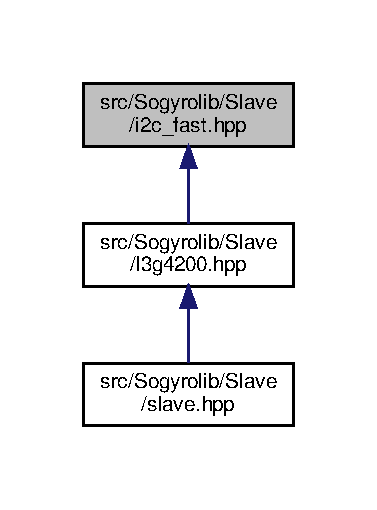
\includegraphics[width=181pt]{i2c__fast_8hpp__dep__incl}
\end{center}
\end{figure}
\subsection*{Classes}
\begin{DoxyCompactItemize}
\item 
class \hyperlink{classi2c__fast}{i2c\+\_\+fast}
\begin{DoxyCompactList}\small\item\em hwlib\+::i2c\+\_\+bus\+\_\+bit\+\_\+banged\+\_\+scl\+\_\+sda Decorator \end{DoxyCompactList}\end{DoxyCompactItemize}

\hypertarget{l3g4200_8hpp}{}\section{src/\+Sogyrolib/\+Slave/l3g4200.hpp File Reference}
\label{l3g4200_8hpp}\index{src/\+Sogyrolib/\+Slave/l3g4200.\+hpp@{src/\+Sogyrolib/\+Slave/l3g4200.\+hpp}}
{\ttfamily \#include \char`\"{}hwlib.\+hpp\char`\"{}}\newline
{\ttfamily \#include \char`\"{}i2c\+\_\+fast.\+hpp\char`\"{}}\newline
Include dependency graph for l3g4200.\+hpp\+:
\nopagebreak
\begin{figure}[H]
\begin{center}
\leavevmode
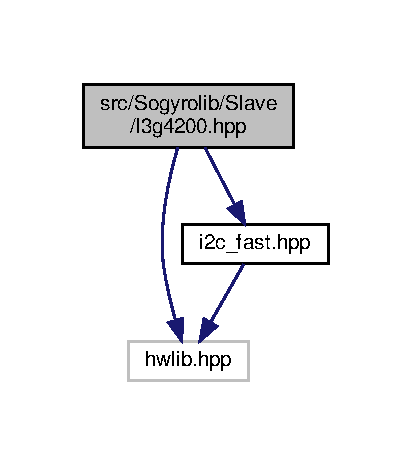
\includegraphics[width=198pt]{l3g4200_8hpp__incl}
\end{center}
\end{figure}
This graph shows which files directly or indirectly include this file\+:
\nopagebreak
\begin{figure}[H]
\begin{center}
\leavevmode
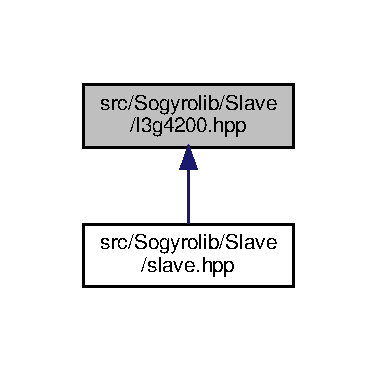
\includegraphics[width=181pt]{l3g4200_8hpp__dep__incl}
\end{center}
\end{figure}
\subsection*{Classes}
\begin{DoxyCompactItemize}
\item 
class \hyperlink{classl3g4200}{l3g4200}
\begin{DoxyCompactList}\small\item\em interface for \hyperlink{classl3g4200}{l3g4200} \end{DoxyCompactList}\end{DoxyCompactItemize}
\subsection*{Macros}
\begin{DoxyCompactItemize}
\item 
\mbox{\Hypertarget{l3g4200_8hpp_a90201d02d51f87225c6241b87262dde5}\label{l3g4200_8hpp_a90201d02d51f87225c6241b87262dde5}} 
\#define {\bfseries S\+C\+A\+L\+E\+\_\+2000}~0x02
\item 
\mbox{\Hypertarget{l3g4200_8hpp_a37e121b2d226ccc3f403f2936aee8dd2}\label{l3g4200_8hpp_a37e121b2d226ccc3f403f2936aee8dd2}} 
\#define {\bfseries S\+C\+A\+L\+E\+\_\+500}~0x01
\item 
\mbox{\Hypertarget{l3g4200_8hpp_a80f3c508fd5519d6e1a30d66499e9797}\label{l3g4200_8hpp_a80f3c508fd5519d6e1a30d66499e9797}} 
\#define {\bfseries S\+C\+A\+L\+E\+\_\+250}~0x00
\end{DoxyCompactItemize}
\subsection*{Functions}
\begin{DoxyCompactItemize}
\item 
void \hyperlink{l3g4200_8hpp_afcc78e012c211becc80ee7d0a43c6edd}{threesixty} (double \&in, double \&out)
\begin{DoxyCompactList}\small\item\em turns data into 360 degrees data \end{DoxyCompactList}\end{DoxyCompactItemize}


\subsection{Function Documentation}
\mbox{\Hypertarget{l3g4200_8hpp_afcc78e012c211becc80ee7d0a43c6edd}\label{l3g4200_8hpp_afcc78e012c211becc80ee7d0a43c6edd}} 
\index{l3g4200.\+hpp@{l3g4200.\+hpp}!threesixty@{threesixty}}
\index{threesixty@{threesixty}!l3g4200.\+hpp@{l3g4200.\+hpp}}
\subsubsection{\texorpdfstring{threesixty()}{threesixty()}}
{\footnotesize\ttfamily void threesixty (\begin{DoxyParamCaption}\item[{double \&}]{in,  }\item[{double \&}]{out }\end{DoxyParamCaption})}



turns data into 360 degrees data 

This function turns givin data and minus data into 360 values for example -\/120 should become 240 and 450 should become 90. 
\hypertarget{slave_8hpp}{}\section{src/\+Sogyrolib/\+Slave/slave.hpp File Reference}
\label{slave_8hpp}\index{src/\+Sogyrolib/\+Slave/slave.\+hpp@{src/\+Sogyrolib/\+Slave/slave.\+hpp}}
{\ttfamily \#include \char`\"{}hwlib.\+hpp\char`\"{}}\newline
{\ttfamily \#include \char`\"{}l3g4200.\+hpp\char`\"{}}\newline
Include dependency graph for slave.\+hpp\+:
\nopagebreak
\begin{figure}[H]
\begin{center}
\leavevmode
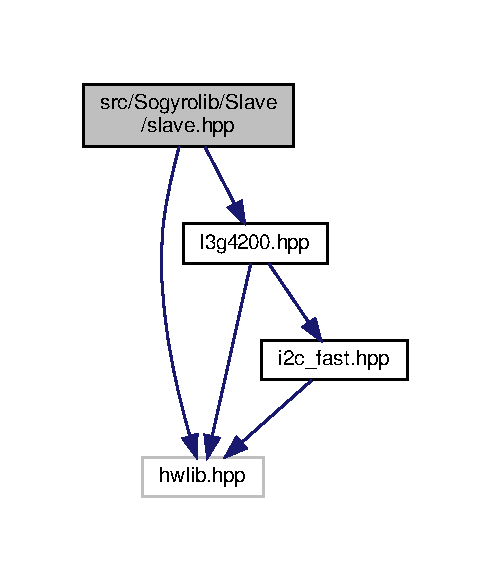
\includegraphics[width=236pt]{slave_8hpp__incl}
\end{center}
\end{figure}
\subsection*{Classes}
\begin{DoxyCompactItemize}
\item 
class \hyperlink{classslave}{slave}
\begin{DoxyCompactList}\small\item\em Class to create a S\+PI slave for Arduino. \end{DoxyCompactList}\end{DoxyCompactItemize}

%--- End generated contents ---

% Index
\backmatter
\newpage
\phantomsection
\clearemptydoublepage
\addcontentsline{toc}{chapter}{Index}
\printindex

\end{document}
